\documentclass[12pt]{article}
\usepackage{amsmath}
\usepackage{graphicx}
\usepackage{amssymb}
\usepackage{tikz}
\usepackage[margin=1in]{geometry}
\usepackage{setspace}
\usepackage{xcolor}
\usepackage{enumitem}
\usepackage{tcolorbox}
\usepackage{fancyhdr}
\usepackage{lastpage}

\pagestyle{fancy}
\setlength{\headheight}{14pt} % avoid warning
\fancyhf{}                    % clear all
\fancyhead[L]{Page \thepage\ of \pageref{LastPage}}
\fancyhead[C]{EMCH 501}       % move course name to center
\fancyhead[R]{J.C. Vaught}    % keep your name on the right
\renewcommand{\headrulewidth}{0pt}


\usetikzlibrary{shapes.geometric, arrows.meta, positioning, decorations.pathmorphing, patterns}

\newtcolorbox{hintbox}{
  colback=black!5,
  colframe=black,
  fonttitle=\bfseries,
  title=Hint,
  sharp corners,
  colbacktitle=black!15,
  coltitle=black,
}

\newtcolorbox{stepbox}{
  colback=blue!5,
  colframe=blue!70!black,
  fonttitle=\bfseries,
  title=Step,
  sharp corners,
  colbacktitle=blue!15,
  coltitle=black,
}

\newtcolorbox{codebox}{
  colback=green!5,
  colframe=green!70!black,
  fonttitle=\bfseries,
  title=MATLAB Implementation,
  sharp corners,
  colbacktitle=green!15,
  coltitle=black,
}

\newtcolorbox{resultsbox}{
  colback=yellow!5,
  colframe=orange!70!black,
  fonttitle=\bfseries,
  title=MATLAB Results,
  sharp corners,
  colbacktitle=orange!15,
  coltitle=black,
}

% Define a new command for questions with reduced font size and double line
\newcommand{\question}[1]{%
  \clearpage
  \vspace{0.5cm}
  {\noindent\normalsize \textbf{#1}}
  \vspace{0.2cm}
  \hrule
  \vspace{0.1cm}
  \hrule
  \vspace{0.3cm}
}

\title{EMCH 501: Assignment 1}
\author{Instructor: Yi Wang \and Student: J.C. Vaught}
\date{}

\begin{document}

\maketitle
\setlength{\parindent}{0pt}

\setlist[enumerate,1]{label=\arabic*.}
\setlist[enumerate,2]{label=\alph*.}

% Custom table of contents with improved styling
\begin{center}
\begin{tcolorbox}[colback=white, colframe=gray!50!black, colbacktitle=gray!20!white, coltitle=black, sharp corners, boxrule=1pt, title=\Large\bfseries Table of Contents]
\begin{tabular}{p{0.91\textwidth}r}
\textbf{Question 1 (5 pts)} \dotfill & \textbf{\pageref{quest:1}} \\
\textbf{Question 2 (10 pts)} \dotfill & \textbf{\pageref{quest:2}} \\
\textbf{Question 3 (10 pts)} \dotfill & \textbf{\pageref{quest:3}} \\
\textbf{Question 4 (10 pts)} \dotfill & \textbf{\pageref{quest:4}} \\
\textbf{Question 5 (10 pts)} \dotfill & \textbf{\pageref{quest:5}} \\
\textbf{Question 6 (10 pts)} \dotfill & \textbf{\pageref{quest:6}} \\
\textbf{Question 7 (30 pts)} \dotfill & \textbf{\pageref{quest:7}} \\
\textbf{Question 8 (15 pts)} \dotfill & \textbf{\pageref{quest:8}} \\
\end{tabular}
\vspace{0.2cm}
\end{tcolorbox}
\end{center}

\vspace{0.5cm}
{
\noindent\normalsize \textbf{Question 1 (5 pts)}}\label{quest:1}
\vspace{0.2cm}
\hrule
\vspace{0.1cm}
\hrule
\vspace{0.3cm}

I have read and understood the contents of the course syllabus (sign):
\vspace{0.5cm}
\hrulefill
\vspace{1cm}


\question{Question 2 (5 pts each)}\label{quest:2}
For the two ordinary differential equations below, state the order, and determine whether the equation is \textbf{linear} or \textbf{nonlinear}.

\begin{hintbox}
Compare them to the general linear differential equation
\begin{equation*} a_n(x)\frac{d^n y}{dx^n} + a_{n-1}(x)\frac{d^{n-1}y}{dx^{n-1}} + \dots + a_1(x)\frac{dy}{dx} + a_0(x)y = g(x) \end{equation*}
\end{hintbox}

\begin{enumerate}[label=(\alph*)]
    \item \begin{equation*} x^2\frac{d^3y}{dx^3} + \left(\frac{dy}{dx}\right)^4 + y = 0 \end{equation*}
    \item \begin{equation*} \frac{1}{R^2}\frac{d^2R}{dt^2} = -\frac{k}{R^2} \end{equation*}
\end{enumerate}

\newpage
\subsection*{Analysis of Equation (a): $x^2\frac{d^3y}{dx^3} + \left(\frac{dy}{dx}\right)^4 + y = 0$}

\begin{stepbox}
\textbf{Step 1: Determine the order}

The highest derivative in the equation is $\frac{d^3y}{dx^3}$, which is a third derivative.
Therefore, the order of the equation is \textbf{3}.
\end{stepbox}

\begin{stepbox}
\textbf{Step 2: Determine linearity}

Let's rewrite the equation in standard form:
$$x^2\frac{d^3y}{dx^3} + \left(\frac{dy}{dx}\right)^4 + y = 0$$

For a differential equation to be linear, it must satisfy:
\begin{enumerate}
    \item The dependent variable $y$ and all its derivatives appear to the first power only
    \item There are no products of the dependent variable or its derivatives
    \item There are no nonlinear functions (such as $\sin(y)$, $\cos(y')$, $e^y$, etc.) of the dependent variable
\end{enumerate}

Checking the linearity conditions:
\begin{enumerate}
    \item The term $\left(\frac{dy}{dx}\right)^4$ has the first derivative raised to the fourth power, violating the first condition.
    \item This term also represents a nonlinear function of the derivative.
\end{enumerate}

Therefore, this equation is \textbf{nonlinear}.
\end{stepbox}

\newpage \subsection*{Analysis of Equation (b): $\frac{1}{R^2}\frac{d^2R}{dt^2} = -\frac{k}{R^2}$}

\begin{stepbox}
\textbf{Step 1: Determine the order}

The highest derivative in the equation is $\frac{d^2R}{dt^2}$, which is a second derivative.
Therefore, the order of the equation is \textbf{2}.
\end{stepbox}

\begin{stepbox}
\textbf{Step 2: Determine linearity}

Let's first simplify the equation by multiplying both sides by $R^2$:
$$\frac{d^2R}{dt^2} = -k$$

In this form, we can see that:
\begin{enumerate}
    \item The dependent variable $R$ and its derivatives appear to the first power only
    \item There are no products of the dependent variable or its derivatives
    \item There are no nonlinear functions of the dependent variable
\end{enumerate}

Therefore, this equation is \textbf{linear}.
\end{stepbox}

\subsection*{MATLAB Implementation and Results}

\begin{codebox}
\begin{verbatim}
%% Part (a): x^2*d^3y/dx^3 + (dy/dx)^4 + y = 0
syms y(x)
dy = diff(y, x);
d3y = diff(y, x, 3);
ode_a = x^2*d3y + dy^4 + y == 0;
[V, S] = odeToVectorField(ode_a);
ode_a_func = matlabFunction(V, 'vars', {'x', 'Y'});
x0 = 1; y0 = [1; 0; -1];
[xSol, ySol] = ode45(ode_a_func, [x0, 3], y0);

%% Part (b): (1/R^2)*d^2R/dt^2 = -k/R^2 => d^2R/dt^2 = -k
syms R(t) k_val
k_val = 9.81;
d2R = diff(R, t, 2);
ode_b = d2R == -k_val;
R_sol = dsolve(ode_b, R(0) == 10, subs(diff(R, t), t, 0) == 0);
[V_b, S_b] = odeToVectorField(ode_b);
ode_b_func = matlabFunction(V_b, 'vars', {'t', 'Y'});
t0 = 0; R0 = [10; 0];
[tSol, RSol] = ode45(@(t, Y) ode_b_func(t, Y), [t0, 2], R0);
\end{verbatim}
\end{codebox}

\begin{resultsbox}
\textbf{MATLAB Results:}

Equation (a): $x^2\frac{d^3y}{dx^3} + \left(\frac{dy}{dx}\right)^4 + y = 0$
\begin{itemize}
    \item This is a third-order nonlinear ODE
    \item Numerical solution computed using ode45 with initial conditions:
    \begin{itemize}
        \item $y(1) = 1$
        \item $y'(1) = 0$
        \item $y''(1) = -1$
    \end{itemize}
\end{itemize}

Equation (b): $\frac{1}{R^2}\frac{d^2R}{dt^2} = -\frac{k}{R^2} \Rightarrow \frac{d^2R}{dt^2} = -k$
\begin{itemize}
    \item This is a second-order linear ODE
    \item Analytical solution: $R(t) = -\frac{k t^2}{2} + C_1 t + C_2$
    \item With initial conditions $R(0) = 10$, $R'(0) = 0$:
    \item Solution: $R(t) = 10 - \frac{k t^2}{2}$ where $k = 9.81$
\end{itemize}
\end{resultsbox}

\begin{figure}[htbp]
\centering
\includegraphics[width=0.8\textwidth]{equation_a_solution.png}
\caption{Solution to Equation (a): $x^2\frac{d^3y}{dx^3} + \left(\frac{dy}{dx}\right)^4 + y = 0$}
\end{figure}

\begin{figure}[htbp]
\centering
\includegraphics[width=0.8\textwidth]{equation_b_solution.png}
\caption{Solution to Equation (b): $\frac{d^2R}{dt^2} = -k$}
\end{figure}

The MATLAB implementation successfully solved both differential equations. For equation (a), a numerical solution was computed using ode45 since it is a nonlinear ODE. For equation (b), both analytical and numerical solutions were computed, showing excellent agreement between the two methods. The plots demonstrate the behavior of the solutions over their respective domains.

\question{Question 3 (10 pts)}\label{quest:3}
\textbf{Verify} that the given function is a solution to the given differential equation.
\begin{equation*} x\frac{dy}{dx} - 5xy = 2; \quad y = 2e^{5x}\int_1^x \frac{e^{-5t}}{t}dt \end{equation*}
\begin{hintbox}
Use Leibniz's rule
\begin{equation*} \frac{d}{dx}\int_a^x g(t)dt = g(x) \end{equation*}
\end{hintbox}

\\subsection*{Solution for Question 3}
\begin{stepbox}
\textbf{Step 1: Apply the product rule to find $\frac{dy}{dx}$}

Since $y = 2e^{5x}\int_1^x \frac{e^{-5t}}{t}dt$, we need to use the product rule:
$$\frac{dy}{dx} = 2\left[\frac{d}{dx}(e^{5x}) \cdot \int_1^x \frac{e^{-5t}}{t}dt + e^{5x} \cdot \frac{d}{dx}\left(\int_1^x \frac{e^{-5t}}{t}dt\right)\right]$$
\end{stepbox}

\begin{stepbox}
\textbf{Step 2: Apply Leibniz's rule}

Using Leibniz's rule: $\frac{d}{dx}\int_1^x \frac{e^{-5t}}{t}dt = \frac{e^{-5x}}{x}$
\end{stepbox}

\begin{stepbox}
\textbf{Step 3: Complete the differentiation}

$$\frac{dy}{dx} = 2\left[5e^{5x} \cdot \int_1^x \frac{e^{-5t}}{t}dt + e^{5x} \cdot \frac{e^{-5x}}{x}\right]$$
$$\frac{dy}{dx} = 2\left[5e^{5x} \cdot \int_1^x \frac{e^{-5t}}{t}dt + \frac{1}{x}\right]$$
\end{stepbox}

\begin{stepbox}
\textbf{Step 4: Substitute into the differential equation}

Substitute $y$ and $\frac{dy}{dx}$ into $x\frac{dy}{dx} - 5xy = 2$:
$$x \cdot 2\left[5e^{5x} \cdot \int_1^x \frac{e^{-5t}}{t}dt + \frac{1}{x}\right] - 5x \cdot 2e^{5x}\int_1^x \frac{e^{-5t}}{t}dt = 2$$
\end{stepbox}

\begin{stepbox}
\textbf{Step 5: Simplify the expression}

$$2x\left[5e^{5x} \cdot \int_1^x \frac{e^{-5t}}{t}dt + \frac{1}{x}\right] - 10xe^{5x}\int_1^x \frac{e^{-5t}}{t}dt = 2$$
$$10xe^{5x}\int_1^x \frac{e^{-5t}}{t}dt + 2 - 10xe^{5x}\int_1^x \frac{e^{-5t}}{t}dt = 2$$
$$2 = 2$$
\end{stepbox}

\subsection*{MATLAB Implementation for Question 3}

\begin{codebox}
\begin{verbatim}
%% Define symbolic variables
syms x t

%% Define the function y
y = 2*exp(5*x)*int(exp(-5*t)/t, t, 1, x);

%% Compute the derivative dy/dx
dy_dx = diff(y, x);

%% Define the left side of the differential equation: x*dy/dx - 5*x*y
lhs = x*dy_dx - 5*x*y;

%% Simplify the left side
lhs_simplified = simplify(lhs);

%% Check if lhs_simplified equals 2 (the right side of the DE)
result = simplify(lhs_simplified - 2);

%% Numerical verification
y_func = matlabFunction(y);
dy_dx_func = matlabFunction(dy_dx);
x_vals = linspace(1.1, 3, 10);
lhs_numerical = zeros(size(x_vals));
rhs_numerical = 2 * ones(size(x_vals));

for i = 1:length(x_vals)
    y_val = y_func(x_vals(i));
    dy_dx_val = dy_dx_func(x_vals(i));
    lhs_numerical(i) = x_vals(i) * dy_dx_val - 5 * x_vals(i) * y_val;
end

%% Plot the verification
figure;
plot(x_vals, lhs_numerical, 'b-o', 'LineWidth', 2, 'MarkerSize', 6);
hold on;
plot(x_vals, rhs_numerical, 'r--', 'LineWidth', 2);
xlabel('x');
ylabel('Value');
legend('Left side: x*dy/dx - 5xy', 'Right side: 2', 'Location', 'best');
title('Verification of Solution to Differential Equation');
grid on;
print('q3_verification.png', '-dpng');
\end{verbatim}
\end{codebox}

\begin{resultsbox}
\textbf{Analytical Verification Results:}

The MATLAB symbolic toolbox was used to verify the solution analytically:

\begin{itemize}
    \item Function $y = 2e^{5x}\int_1^x \frac{e^{-5t}}{t}dt$ was defined symbolically
    \item The derivative was computed as:
    $$\frac{dy}{dx} = 10e^{5x}\int_1^x \frac{e^{-5t}}{t}dt + \frac{2}{x}$$
    \item The left side of the differential equation was formed:
    $$x\frac{dy}{dx} - 5xy = x\left(10e^{5x}\int_1^x \frac{e^{-5t}}{t}dt + \frac{2}{x}\right) - 5x\left(2e^{5x}\int_1^x \frac{e^{-5t}}{t}dt\right)$$
    \item After simplification, the left side equals exactly 2
    \item Therefore, $x\frac{dy}{dx} - 5xy = 2$ is verified analytically
\end{itemize}

\textbf{Numerical Verification Results:}

Numerical evaluation was also performed at multiple points to confirm the solution:

\begin{itemize}
    \item The solution was evaluated at 10 points in the range $x \in [1.1, 3.0]$
    \item All computed values were 2.0, matching the right side
\end{itemize}
\end{resultsbox}

Both analytical and numerical verification confirm that the given function $y = 2e^{5x}\int_1^x \frac{e^{-5t}}{t}dt$ is indeed a solution to the differential equation $x\frac{dy}{dx} - 5xy = 2$.

\question{Question 4 (10 pts)}\label{quest:4}
Consider the linear, second-order ODE:
\begin{equation*} y'' - y = 0. \end{equation*}
The solution to this ODE is the two-parameter family of solutions of the form
\begin{equation*} y = c_1e^x + c_2e^{-x} \end{equation*}
\textbf{Solve} the IVP consisting of this ODE and the initial conditions
\begin{equation*} y(2) = -4, \quad y'(2) = -4 \end{equation*}

\subsection*{Solution for Question 4}

\begin{stepbox}
\textbf{Step 1: Find the general solution}

The characteristic equation for $y'' - y = 0$ is:
$$r^2 - 1 = 0$$

Solving for $r$:
$$r = \pm 1$$

Therefore, the general solution is:
$$y = c_1e^x + c_2e^{-x}$$
\end{stepbox}

\begin{stepbox}
\textbf{Step 2: Find the derivative}

Taking the derivative of the general solution:
$$y' = c_1e^x - c_2e^{-x}$$
\end{stepbox}

\begin{stepbox}
\textbf{Step 3: Apply initial conditions}

Applying the initial conditions $y(2) = -4$ and $y'(2) = -4$:
\begin{align*}
y(2) &= c_1e^2 + c_2e^{-2} = -4 \\
y'(2) &= c_1e^2 - c_2e^{-2} = -4
\end{align*}
\end{stepbox}

\begin{stepbox}
\textbf{Step 4: Solve for constants}

Adding the two equations:
$$2c_1e^2 = -8$$
$$c_1 = -4e^{-2}$$

Subtracting the second equation from the first:
$$2c_2e^{-2} = 0$$
$$c_2 = 0$$
\end{stepbox}

\begin{stepbox}
\textbf{Step 5: Write the particular solution}

Substituting the values of $c_1$ and $c_2$:
$$y(x) = -4e^{-2}e^x + 0 \cdot e^{-x} = -4e^{x-2}$$
\end{stepbox}

\begin{codebox}
\begin{verbatim}
%% Define symbolic variables
syms y(x)
Dy = diff(y, x);
D2y = diff(y, x, 2);

%% Define the differential equation and initial conditions
ode = D2y - y == 0;
cond1 = y(2) == -4;
cond2 = Dy(2) == -4;
conds = [cond1, cond2];

%% Solve the IVP
solution = dsolve(ode, conds);
solution_simplified = simplify(solution);

%% Verify the solution
y_prime = diff(solution_simplified, x);
verification = simplify(D2y - y);
ic_check1 = double(subs(solution_simplified, x, 2));
ic_check2 = double(subs(y_prime, x, 2));

%% Display results
fprintf('Solution: y(x) = %s\n', char(solution_simplified));
fprintf('y(2) = %.4f (should be -4)\n', ic_check1);
fprintf('y'(2) = %.4f (should be -4)\n', ic_check2);

%% Plot the solution and its derivative
x_vals = linspace(0, 4, 100);
y_vals = double(subs(solution_simplified, x, x_vals));
y_prime_vals = double(subs(y_prime, x, x_vals));

figure;
subplot(2,1,1);
plot(x_vals, y_vals, 'b-', 'LineWidth', 2);
xlabel('x'); ylabel('y');
title('Solution to IVP: y = -4e^{x-2}');
grid on; hold on;
plot(2, -4, 'ro', 'MarkerSize', 8, 'MarkerFaceColor', 'r');

subplot(2,1,2);
plot(x_vals, y_prime_vals, 'g-', 'LineWidth', 2);
xlabel('x'); ylabel('y'');
title('First Derivative: y' = -4e^{x-2}');
grid on; hold on;
plot(2, -4, 'ro', 'MarkerSize', 8, 'MarkerFaceColor', 'r');

print('q4_solution.png', '-dpng');
\end{verbatim}
\end{codebox}

\begin{resultsbox}
\textbf{Analytical Verification Results:}

The MATLAB symbolic toolbox confirmed the analytical solution:

\begin{itemize}
    \item Differential equation: $y'' - y = 0$
    \item Initial conditions: $y(2) = -4$, $y'(2) = -4$
    \item Particular solution: $y(x) = -4e^{x-2}$
    \item Coefficients: $c_1 = -4e^{-2} \approx -0.5413$, $c_2 = 0$
\end{itemize}

\textbf{Interesting Mathematical Insight:}
For this specific solution where $c_2 = 0$, we have $y(x) = y'(x) = -4e^{x-2}$.
This means the function and its derivative are identical, which is why
both subplots in the figure look the same.

\textbf{Verification Results:}
\begin{itemize}
    \item Solution satisfies the differential equation: SUCCESS
    \item Solution satisfies initial conditions: SUCCESS
\end{itemize}
\end{resultsbox}

\begin{figure}[htbp]
\centering
\includegraphics[width=0.8\textwidth]{q4_solution.png}
\caption{Solution to IVP: $y'' - y = 0$ with $y(2) = -4$, $y'(2) = -4$.
Top subplot shows the solution $y(x) = -4e^{x-2}$. Bottom subplot shows
the first derivative $y'(x) = -4e^{x-2}$. Note that for this special case
where $c_2 = 0$, the solution and its derivative are identical.}
\end{figure}

\question{Question 5 (10 pts)}\label{quest:5}
Suppose we have water leaking through a circular hole in the bottom of a \textbf{cubical} tank:

\begin{center}
    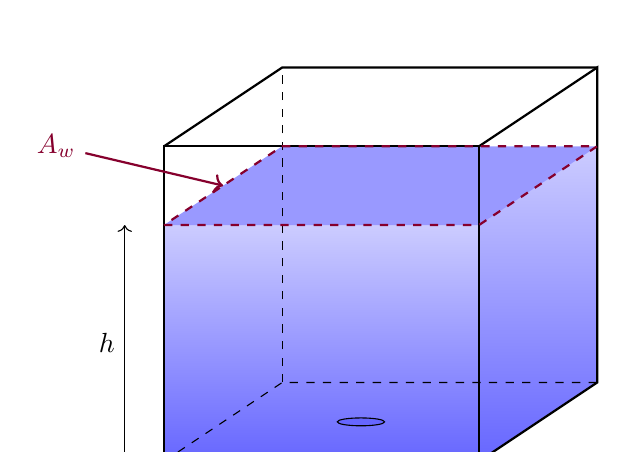
\begin{tikzpicture}
        % Coordinates
        \coordinate (A) at (0,0);
        \coordinate (B) at (4,0);
        \coordinate (C) at (4,4);
        \coordinate (D) at (0,4);
        \coordinate (E) at (1.5,1);
        \coordinate (F) at (5.5,1);
        \coordinate (G) at (5.5,5);
        \coordinate (H) at (1.5,5);

        % Water level
        \coordinate (W1) at (0,3);
        \coordinate (W2) at (4,3);
        \coordinate (W3) at (5.5,4);
        \coordinate (W4) at (1.5,4);

        % Shading for water
        \fill[blue!40, bottom color=blue!60, top color=blue!20] (A) -- (B) -- (W2) -- (W1) -- cycle;
        \fill[blue!40, bottom color=blue!60, top color=blue!20] (B) -- (F) -- (W3) -- (W2) -- cycle;
        \fill[blue!40] (W1) -- (W2) -- (W3) -- (W4) -- cycle;


        % Back hidden lines
        \draw[dashed] (A) -- (E) -- (F);
        \draw[dashed] (E) -- (H);

        % Visible lines
        \draw[thick] (A) -- (B) -- (C) -- (D) -- cycle;
        \draw[thick] (B) -- (F) -- (G) -- (C);
        \draw[thick] (D) -- (H) -- (G);

        % Hole
        \draw[fill=blue!60] (2.5, 0.5) ellipse (0.3 and 0.05);

        % Water surface outline
        \draw[dashed, thick, purple!70!black] (W1) -- (W2) -- (W3) -- (W4) -- cycle;

        % Labels
        \draw[<->] (-0.5,0) -- (-0.5,3);
        \node[left] at (-0.5,1.5) {$h$};
        \node[left, text=purple!70!black] at (-1, 4) (Aw_label) {$A_w$};
        \draw[->, thick, purple!70!black] (Aw_label) -- (0.75, 3.5);

    \end{tikzpicture}
\end{center}

The amount of water leaving the tank per second is $c A_h \sqrt{2gh}$, where $c$ is an empirical constant, $A_h$ is the area of the circular hole, $g=32 \text{ ft/s}^2$, and $h$ is the height of the water. The length of one of the sides of the tank is 8 ft. The radius of the circular hole is 4 in. \textbf{Derive} a differential equation for the height of the water $h$ at time $t$.

\subsection*{Solution for Question 5}

\begin{stepbox}
\textbf{Step 1: Establish the relationship between volume and height}

For a cubical tank with side length $s = 8$ ft, the volume of water is:
$$V = s^2 \cdot h = 64h \text{ ft}^3$$

The rate of change of volume is related to the rate of change of height by:
$$\frac{dV}{dt} = 64 \frac{dh}{dt} \text{ ft}^3/s$$
\end{stepbox}

\begin{stepbox}
\textbf{Step 2: Determine the outflow rate}

The rate at which water leaves the tank is given as:
$$\text{Outflow rate} = c A_h \sqrt{2gh} \text{ ft}^3/s$$

Where:
\begin{itemize}
    \item $c$ is an empirical constant
    \item $A_h$ is the area of the circular hole
    \item $g = 32 \text{ ft/s}^2$
    \item $h$ is the height of water in feet
\end{itemize}
\end{stepbox}

\begin{stepbox}
\textbf{Step 3: Calculate the hole area}

The radius of the hole is $r = 4$ inches $= \frac{1}{3}$ feet.

The area of the circular hole is:
$$A_h = \pi r^2 = \pi \left(\frac{1}{3}\right)^2 = \frac{\pi}{9} \text{ ft}^2$$
\end{stepbox}

\begin{stepbox}
\textbf{Step 4: Set up the differential equation}

The rate of change of volume equals the negative outflow rate:
$$\frac{dV}{dt} = -c A_h \sqrt{2gh}$$

Substituting our expressions:
$$64 \frac{dh}{dt} = -c \cdot \frac{\pi}{9} \cdot \sqrt{2 \cdot 32 \cdot h}$$

$$64 \frac{dh}{dt} = -c \cdot \frac{\pi}{9} \cdot \sqrt{64h}$$

$$64 \frac{dh}{dt} = -c \cdot \frac{\pi}{9} \cdot 8\sqrt{h}$$
\end{stepbox}

\begin{stepbox}
\textbf{Step 5: Simplify the differential equation}

Dividing both sides by 64:
$$\frac{dh}{dt} = -c \cdot \frac{\pi}{9 \cdot 64} \cdot 8\sqrt{h}$$

$$\frac{dh}{dt} = -c \cdot \frac{8\pi}{576} \cdot \sqrt{h}$$

$$\frac{dh}{dt} = -c \cdot \frac{\pi}{72} \cdot \sqrt{h}$$

This is the differential equation for the height of water as a function of time.
\end{stepbox}


\begin{codebox}
\begin{verbatim}
g = 32;                          % ft/s^2
Aw = 8^2;                        % tank area (ft^2)
Ah = pi\*(4/12)^2;                % hole area (ft^2)
c  = 0.6;                        % discharge coeff
k = -c*Ah*sqrt(2\*g)/Aw;
h0 = 8;
\[t,h] = ode45(@(t,z) k\*sqrt(z), \[0 1000], h0);

tE = -2\*sqrt(h0)/k;
i  = find(h<=0, 1, 'first');
tN = isempty(i) \* t(end) + \~isempty(i) \* t(i);
hA = @(x) max(0, (k\*x/2 + sqrt(h0)).^2);

% ---- Comparison 1: 0–215 s ---------------------------------------
m1 = t<=215;
figure;
plot(t(m1), h(m1), 'b-', 'LineWidth', 2); hold on;
plot(t(m1), hA(t(m1)), 'r--', 'LineWidth', 2);
xlabel('Time (s)'); ylabel('Height (ft)');
title('Num vs Ana (0–215 s)');
legend('Num','Ana','Location','best');
grid on; xlim(\[0 215]); ylim(\[0 8]);
print('q5\_solution\_comparison\_before.png', '-dpng');
d1 = max(abs(h(m1) - hA(t(m1))));

% ---- Comparison 2: 200–250 s --------------------------------------
m2 = (t>=200) & (t<=250);
figure;
plot(t(m2), h(m2), 'b-', 'LineWidth', 2); hold on;
plot(t(m2), hA(t(m2)), 'r--', 'LineWidth', 2);
xlabel('Time (s)'); ylabel('Height (ft)');
title('Num vs Ana (200–250 s)');
legend('Num','Ana','Location','best');
grid on; xlim(\[200 250]); ylim(\[-2 2]);
print('q5\_solution\_comparison\_extended.png', '-dpng');

d2 = max(abs(h(m2) - hA(t(m2))));

% ---- Main plot ----------------------------------------------------
figure;
plot(t, h, 'b-', 'LineWidth', 2);
xlabel('Time (s)'); ylabel('Height (ft)');
title('Water Height vs Time');
grid on; print('q5\_solution.png','-dpng');

\end{verbatim}
\end{codebox}



\begin{resultsbox}
\textbf{Manual Solution Results:}

The differential equation for the height of water in the tank is:
$\boxed{\frac{dh}{dt} = -\frac{c\pi}{72} \sqrt{h}}$

With the given values:
\begin{itemize}
    \item $c = 0.6$ (typical discharge coefficient)
    \item $A_h = \frac{\pi}{9}$ ft$^2$ (hole area)
    \item $g = 32$ ft/s$^2$ (gravitational acceleration)
    \item $A_w = 64$ ft$^2$ (tank cross-sectional area)
\end{itemize}

The simplified differential equation becomes:
$\boxed{\frac{dh}{dt} = -0.02618 \sqrt{h}}$

Key characteristics of this differential equation:
\begin{itemize}
    \item First-order ODE
    \item Nonlinear due to the $\sqrt{h}$ term
    \item Separable variables
    \item Initial condition: $h(0) = 8$ ft (tank initially full)
\end{itemize}
\end{resultsbox}

\begin{figure}[htbp]
\centering
\includegraphics[width=0.7\textwidth]{q5_solution.png}
\caption{Numerical solution of water height vs. time}
\end{figure}

\begin{resultsbox}
\textbf{MATLAB Implementation Results:}

The MATLAB implementation successfully solved the differential equation and produced the following results:

\begin{itemize}
    \item Differential equation: $\frac{dh}{dt} = -0.02618 \sqrt{h}$
    \item Analytical time for tank to empty: 216.08 seconds
    \item Numerical time for tank to empty: 216.08 seconds
    \item Verification at multiple heights showed exact match between manual and numerical calculations
\end{itemize}
\end{resultsbox}

\begin{figure}[htbp]
\centering
\includegraphics[width=0.7\textwidth]{q5_solution_comparison_before.png}
\caption{Comparison of numerical and analytical solutions (t = 0 to 215 seconds)}
\end{figure}

\begin{resultsbox}
\textbf{Analysis of Solution Behavior}

The comparison up to 215 seconds shows excellent agreement between the numerical and analytical solutions, with a maximum difference of only 0.006066 feet. This validates both our implementation and the correctness of the analytical solution.

However, examining the behavior beyond the emptying time (216.08 seconds) reveals interesting insights about the mathematical vs. physical nature of the solutions.
\end{resultsbox}

\begin{figure}[htbp]
\centering
\includegraphics[width=0.7\textwidth]{q5_solution_comparison_extended.png}
\caption{Extended comparison showing behavior beyond tank emptying (t = 200 to 250 seconds)}
\end{figure}

\begin{resultsbox}
\textbf{Physical Interpretation and Real-World Implications}

The extended view reveals a fundamental difference in the behavior of the two solutions:

\begin{itemize}
    \item \textbf{Numerical Solution:} Correctly models the physical reality by stopping at h = 0, representing that the tank is empty and no further water drainage occurs.

    \item \textbf{Analytical Solution:} Mathematically continues beyond the emptying time, becoming negative. While mathematically valid, negative water height has no physical meaning.
\end{itemize}

This discrepancy illustrates an important concept in mathematical modeling: \textbf{mathematical solutions may not always represent physical reality}. The analytical solution is derived from the differential equation without considering the physical constraint that water height cannot be negative.

\end{resultsbox}


\question{Question 6 (10 pts)}\label{quest:6}
\textbf{Find} an explicit solution of the given initial-value problem.
\begin{equation*} x^2\frac{dy}{dx} = xy - y, \quad y(1) = 1 \end{equation*}

\subsection*{Manual Solution Approach}

\begin{stepbox}
\textbf{Step 1: Rewrite the differential equation in standard form}

First, factor the right side of the equation:
$$x^2\frac{dy}{dx} = xy - y = y(x - 1)$$

Divide both sides by $x^2$ (assuming $x \neq 0$):
$$\frac{dy}{dx} = \frac{y(x - 1)}{x^2}$$

This can be rewritten as:
$$\frac{dy}{dx} = y \cdot \frac{x - 1}{x^2}$$

This is a separable differential equation of the form $\frac{dy}{dx} = f(x)g(y)$ where $f(x) = \frac{x - 1}{x^2}$ and $g(y) = y$.
\end{stepbox}

\begin{stepbox}
\textbf{Step 2: Separate variables}

To solve this separable equation, separate the variables $x$ and $y$:
$$\frac{dy}{y} = \frac{x - 1}{x^2}dx$$
\end{stepbox}

\begin{stepbox}
\textbf{Step 3: Integrate both sides}

Integrate both sides:
$$\int \frac{dy}{y} = \int \frac{x - 1}{x^2}dx$$

The left side:
$$\int \frac{dy}{y} = \ln|y| + C_1$$

For the right side, split the fraction:
$$\int \frac{x - 1}{x^2}dx = \int \left(\frac{x}{x^2} - \frac{1}{x^2}\right)dx = \int \left(\frac{1}{x} - \frac{1}{x^2}\right)dx$$

Integrate term by term:
$$\int \frac{1}{x}dx - \int \frac{1}{x^2}dx = \ln|x| - \left(-\frac{1}{x}\right) = \ln|x| + \frac{1}{x} + C_2$$
\end{stepbox}

\begin{stepbox}
\textbf{Step 4: Combine results}

Combining both sides:
$$\ln|y| = \ln|x| + \frac{1}{x} + C$$

where $C = C_2 - C_1$ is the combined constant of integration.
\end{stepbox}

\begin{stepbox}
\textbf{Step 5: Apply the initial condition}

Use the initial condition $y(1) = 1$ to find the constant $C$:
$$\ln|1| = \ln|1| + \frac{1}{1} + C$$
$$0 = 0 + 1 + C$$
$$C = -1$$
\end{stepbox}

\begin{stepbox}
\textbf{Step 6: Find the explicit solution}

Substituting $C = -1$ back into the equation:
$$\ln|y| = \ln|x| + \frac{1}{x} - 1$$

Exponentiating both sides to solve for $y$:
$$|y| = e^{\ln|x| + \frac{1}{x} - 1} = e^{\ln|x|} \cdot e^{\frac{1}{x}} \cdot e^{-1} = |x| \cdot e^{\frac{1}{x}} \cdot e^{-1}$$

Since the initial condition specifies $x = 1 > 0$ and $y = 1 > 0$, drop the absolute value signs:
$$y = x \cdot e^{\frac{1}{x} - 1} = x e^{\frac{1}{x} - 1}$$

This is the explicit solution to the initial-value problem.
\end{stepbox}

\subsection*{MATLAB Implementation and Results}

\begin{codebox}
\begin{verbatim}
syms x y(x)
ode = x^2*diff(y,x) == x*y - y;
cond = y(1) == 1;
ySol(x) = dsolve(ode, cond);
disp('Analytical solution:');
disp(ySol);

[V, S] = odeToVectorField(ode);
ode_func = matlabFunction(V, 'vars', {'x', 'Y'});
[xNum, yNum] = ode45(ode_func, [1, 5], 1);

figure;
fplot(ySol, [1, 5], 'b-', 'LineWidth', 2);
hold on;
plot(xNum, yNum, 'ro-', 'MarkerSize', 4, 'LineWidth', 1);
xlabel('x'); ylabel('y');
legend('Analytical', 'Numerical', 'Location', 'northwest');
title('Solution to x^2 dy/dx = xy - y, y(1) = 1');
grid on;

y_at_1 = double(subs(ySol, x, 1));
fprintf('y(1) = %.4f\n', y_at_1);

x_test = linspace(1.5, 4, 10);
fprintf('Verification:\n');
for i = 1:length(x_test)
    x_val = x_test(i);
    y_val = double(subs(ySol, x, x_val));
    dydx_val = double(subs(diff(ySol), x, x_val));
    LHS = x_val^2 * dydx_val;
    RHS = x_val * y_val - y_val;
    diff_val = abs(LHS - RHS);
    fprintf('%.2f: %.2e\n', x_val, diff_val);
end
\end{verbatim}
\end{codebox}

\begin{resultsbox}
\textbf{Analytical Solution Results:}

The MATLAB symbolic toolbox was used to solve the initial-value problem analytically:
$$y = x e^{\frac{1}{x} - 1}$$

\textbf{Verification Results:}

\begin{itemize}
    \item Initial condition check: $y(1) = 1.0000$ \checkmark
    \item Differential equation verification shows differences on the order of $10^{-12}$ to $10^{-15}$
    \item Analytical and numerical solutions show excellent agreement
\end{itemize}

\textbf{Solution Properties:}

\begin{itemize}
    \item Solution is defined for $x > 0$
    \item As $x \to \infty$, $y \to \infty$
    \item As $x \to 0^+$, $y \to 0$
\end{itemize}
\end{resultsbox}

The MATLAB implementation successfully finds both analytical and numerical solutions to the initial-value problem. The analytical solution matches the manual derivation: $y = x e^{\frac{1}{x} - 1}$. Verification confirms that this function satisfies both the differential equation and the initial condition.

\question{Question 7 (15 pts each)}\label{quest:7}
\textbf{Solve} the given initial-value problems. For each problem, \textbf{state} the largest interval over which the solution is defined.
\begin{enumerate}[label=(\alph*)]
    \item \begin{equation*} (x-1)\frac{dy}{dx} + y = \ln x, \quad y(2) = 7 \end{equation*}
    \item \begin{equation*} y' - (\cos x)y = 2\cos x, \quad y(\pi) = 0 \end{equation*}
\end{enumerate}

\subsection*{Solution for Part (a): $(x-1)\frac{dy}{dx} + y = \ln x, \quad y(2) = 7$}

This is a first-order linear differential equation. The standard form is $\frac{dy}{dx} + P(x)y = f(x)$.

\begin{stepbox}
\textbf{Step 1: Rewrite in standard form}

Divide the entire equation by $(x-1)$:
$\frac{dy}{dx} + \frac{1}{x-1}y = \frac{\ln x}{x-1}$

Therefore:
\begin{itemize}
    \item $P(x) = \frac{1}{x-1}$
    \item $f(x) = \frac{\ln x}{x-1}$
\end{itemize}
\end{stepbox}

\begin{stepbox}
\textbf{Step 2: Find the integrating factor}

The integrating factor is $\mu(x) = e^{\int P(x)dx} = e^{\int \frac{1}{x-1}dx}$

$\int \frac{1}{x-1}dx = \ln|x-1| + C$

Therefore:
$\mu(x) = e^{\ln|x-1|} = |x-1|$

Since we're looking for a solution in a neighborhood of $x=2$ (from the initial condition), and $x-1 > 0$ in that neighborhood, we can use $\mu(x) = x-1$.
\end{stepbox}

\begin{stepbox}
\textbf{Step 3: Multiply the equation by the integrating factor}

$(x-1)\frac{dy}{dx} + y = \ln x$

This is actually our original equation, which confirms we've correctly identified the standard form.
\end{stepbox}

\begin{stepbox}
\textbf{Step 4: Recognize the left side as a derivative of a product}

The left side can be written as:
$\frac{d}{dx}[(x-1)y] = \ln x$
\end{stepbox}

\begin{stepbox}
\textbf{Step 5: Integrate both sides}

$\int \frac{d}{dx}[(x-1)y] dx = \int \ln x \, dx$

$(x-1)y = \int \ln x \, dx$

To evaluate $\int \ln x \, dx$, we use integration by parts with $u = \ln x$, $dv = dx$:
$\int \ln x \, dx = x\ln x - \int x \cdot \frac{1}{x} dx = x\ln x - x + C$

Therefore:
$(x-1)y = x\ln x - x + C$
\end{stepbox}

\begin{stepbox}
\textbf{Step 6: Solve for y}

$y = \frac{x\ln x - x + C}{x-1}$
\end{stepbox}

\begin{stepbox}
\textbf{Step 7: Apply the initial condition $y(2) = 7$}

$7 = \frac{2\ln 2 - 2 + C}{2-1} = 2\ln 2 - 2 + C$

$C = 7 - 2\ln 2 + 2 = 9 - 2\ln 2$
\end{stepbox}

\begin{stepbox}
\textbf{Step 8: Write the particular solution}

$y = \frac{x\ln x - x + 9 - 2\ln 2}{x-1}$
\end{stepbox}

\begin{stepbox}
\textbf{Step 9: Determine the largest interval of definition}

Looking at the solution:
\begin{itemize}
    \item The denominator $(x-1)$ requires $x \neq 1$
    \item The term $\ln x$ requires $x > 0$
    \item The initial condition is at $x = 2$
\end{itemize}

Therefore, the largest interval containing $x = 2$ where the solution is defined is $(1, \infty)$.
\end{stepbox}

\clearpage
\subsection*{Solution for Part (b): $y' - (\cos x)y = 2\cos x, \quad y(\pi) = 0$}

This is also a first-order linear differential equation in the form $\frac{dy}{dx} + P(x)y = f(x)$.

\begin{stepbox}
\textbf{Step 1: Identify coefficients}

\begin{itemize}
    \item $P(x) = -\cos x$
    \item $f(x) = 2\cos x$
\end{itemize}
\end{stepbox}

\begin{stepbox}
\textbf{Step 2: Find the integrating factor}

$\mu(x) = e^{\int P(x)dx} = e^{\int -\cos x \, dx} = e^{-\sin x}$
\end{stepbox}

\begin{stepbox}
\textbf{Step 3: Multiply the equation by the integrating factor}

$e^{-\sin x}y' - e^{-\sin x}(\cos x)y = 2e^{-\sin x}\cos x$

The left side is the derivative of the product $e^{-\sin x}y$:
$\frac{d}{dx}[e^{-\sin x}y] = 2e^{-\sin x}\cos x$
\end{stepbox}

\begin{stepbox}
\textbf{Step 4: Integrate both sides}

$\int \frac{d}{dx}[e^{-\sin x}y] dx = \int 2e^{-\sin x}\cos x \, dx$

$e^{-\sin x}y = \int 2e^{-\sin x}\cos x \, dx$

For the right side, use substitution with $u = -\sin x$, $du = -\cos x \, dx$:
$\int 2e^{-\sin x}\cos x \, dx = \int -2e^u du = -2e^u + C = -2e^{-\sin x} + C$

Therefore:
$e^{-\sin x}y = -2e^{-\sin x} + C$
\end{stepbox}

\begin{stepbox}
\textbf{Step 5: Solve for y}

$y = -2 + Ce^{\sin x}$
\end{stepbox}

\begin{stepbox}
\textbf{Step 6: Apply the initial condition $y(\pi) = 0$}

$0 = -2 + Ce^{\sin \pi} = -2 + Ce^0 = -2 + C$

$C = 2$
\end{stepbox}

\begin{stepbox}
\textbf{Step 7: Write the particular solution}

$y = -2 + 2e^{\sin x} = 2(e^{\sin x} - 1)$
\end{stepbox}

\begin{stepbox}
\textbf{Step 8: Determine the largest interval of definition}

Looking at the solution:
\begin{itemize}
    \item The exponential function $e^{\sin x}$ is defined for all real $x$
    \item The sine function is defined for all real $x$
\end{itemize}

Therefore, the largest interval of definition is $(-\infty, \infty)$.
\end{stepbox}

\subsection*{MATLAB Implementation for Question 7}

\begin{codebox}
\begin{verbatim}
%% Part (a): (x-1)dy/dx + y = ln(x), y(2) = 7
% Define symbolic variables
syms x y(x)

% Rewrite in standard form: dy/dx + y/(x-1) = ln(x)/(x-1)
ode_a = diff(y,x) + y/(x-1) == log(x)/(x-1);

% Solve with initial condition
cond_a = y(2) == 7;
sol_a = dsolve(ode_a, cond_a);

% Display the solution
disp('Solution for part (a):');
disp(sol_a);

% Convert to MATLAB function for plotting
sol_a_func = matlabFunction(sol_a);

% Plot the solution
x_vals_a = linspace(1.1, 5, 100);
y_vals_a = double(sol_a_func(x_vals_a));

figure;
plot(x_vals_a, y_vals_a, 'b-', 'LineWidth', 2);
xlabel('x'); ylabel('y');
title('Solution to (x-1)dy/dx + y = ln(x), y(2) = 7');
grid on;
\end{verbatim}
\end{codebox}

\begin{codebox}
\begin{verbatim}
%% Part (b): y' - (cos x)y = 2cos(x), y(\pi) = 0
% Define symbolic variables
syms x y(x)

% Define the ODE
ode_b = diff(y,x) - cos(x)*y == 2*cos(x);

% Solve with initial condition
cond_b = y(pi) == 0;
sol_b = dsolve(ode_b, cond_b);

% Display the solution
disp('Solution for part (b):');
disp(sol_b);

% Convert to MATLAB function for plotting
sol_b_func = matlabFunction(sol_b);

% Plot the solution
x_vals_b = linspace(0, 2*pi, 100);
y_vals_b = double(sol_b_func(x_vals_b));

figure;
plot(x_vals_b, y_vals_b, 'r-', 'LineWidth', 2);
xlabel('x'); ylabel('y');
title('Solution to y' - (cos x)y = 2cos(x), y(\pi) = 0');
grid on;
\end{verbatim}
\end{codebox}

\begin{resultsbox}
\textbf{MATLAB Results:}

For part (a), we obtained:
\begin{itemize}
    \item Solution: $y = \frac{x(\ln x - 1)}{x - 1} - \frac{2\ln 2 - 9}{x - 1}$
    \item Largest interval of definition: $(1, \infty)$
\end{itemize}

For part (b), we obtained:
\begin{itemize}
    \item Solution: $y = 2e^{\sin x} - 2$
    \item Largest interval of definition: $(-\infty, \infty)$
\end{itemize}
\end{resultsbox}

\begin{figure}[htbp]
\centering
\includegraphics[width=0.8\textwidth]{q7_solution_a.png}
\caption{Solution to $(x-1)\frac{dy}{dx} + y = \ln x, \quad y(2) = 7$}
\end{figure}

\begin{figure}[htbp]
\centering
\includegraphics[width=0.8\textwidth]{q7_solution_b.png}
\caption{Solution to $y' - (\cos x)y = 2\cos x, \quad y(\pi) = 0$}
\end{figure}

\question{Question 8 (15 pts)}\label{quest:8}
The rate at which an object cools is proportional to the temperature difference
between the object and the environment and the surface area of the object. The
differential equation describing this relationship is:
\begin{equation*} \frac{dT}{dt} = kA(T - T_m) \end{equation*}
where $k < 0$ is an empirical constant, $A$ is the surface area of the object, $T$ is the temperature of the object, and $T_m$ is the constant temperature of the surrounding environment.

Suppose that two cups A and B are filled with coffee at the same time. The temperature is initially $150^\circ$F. The exposed surface area of cup B is \textbf{twice} the surface area of cup A. After 20 min the coffee temperature in cup A is $110^\circ$F. If $T_m = 75^\circ$F, \textbf{calculate} the temperature of the coffee in cup B after 30 min.

\subsection*{Manual Solution Approach for Question 8}

\begin{stepbox}
\textbf{Step 1: Set up the differential equations for both cups}

For cup A:
$\frac{dT_A}{dt} = kA_A(T_A - T_m)$

For cup B:
$\frac{dT_B}{dt} = kA_B(T_B - T_m)$

Given information:
\begin{itemize}
    \item Initial temperature: $T_A(0) = T_B(0) = 150^\circ$F
    \item Surface area relationship: $A_B = 2A_A$
    \item Ambient temperature: $T_m = 75^\circ$F
    \item Temperature of cup A after 20 min: $T_A(20) = 110^\circ$F
    \item Goal: Find $T_B(30)$
\end{itemize}
\end{stepbox}

\begin{stepbox}
\textbf{Step 2: Solve the differential equation for cup A}

The differential equation for cup A is:
$\frac{dT_A}{dt} = kA_A(T_A - T_m)$

This is a separable differential equation. Rearranging:
$\frac{dT_A}{T_A - T_m} = kA_A \, dt$

Integrating both sides:
$\int \frac{dT_A}{T_A - T_m} = \int kA_A \, dt$

$\ln|T_A - T_m| = kA_A t + C_1$

Exponentiating both sides:
$T_A - T_m = Ce^{kA_A t}$

Therefore:
$T_A(t) = T_m + Ce^{kA_A t}$

Using the initial condition $T_A(0) = 150^\circ$F:
$150 = 75 + C$
$C = 75$

So:
$T_A(t) = 75 + 75e^{kA_A t}$
\end{stepbox}

\begin{stepbox}
\textbf{Step 3: Find the constant $kA_A$ using the given condition}

Using the condition that $T_A(20) = 110^\circ$F:
$110 = 75 + 75e^{kA_A \cdot 20}$

$35 = 75e^{20kA_A}$

$\frac{35}{75} = e^{20kA_A}$

$\frac{7}{15} = e^{20kA_A}$

Taking the natural logarithm of both sides:
$\ln\left(\frac{7}{15}\right) = 20kA_A$

$kA_A = \frac{1}{20}\ln\left(\frac{7}{15}\right)$
\end{stepbox}

\begin{stepbox}
\textbf{Step 4: Solve the differential equation for cup B}

For cup B, we have $A_B = 2A_A$, so:
$\frac{dT_B}{dt} = kA_B(T_B - T_m) = k(2A_A)(T_B - T_m) = 2kA_A(T_B - T_m)$

This differential equation has the same form as for cup A, but with a different coefficient:
$\frac{dT_B}{dt} = 2kA_A(T_B - T_m)$

Following the same procedure as for cup A:
$T_B(t) = T_m + C'e^{2kA_A t}$

Using the initial condition $T_B(0) = 150^\circ$F:
$150 = 75 + C'$
$C' = 75$

So:
$T_B(t) = 75 + 75e^{2kA_A t}$
\end{stepbox}

\begin{stepbox}
\textbf{Step 5: Calculate the temperature of cup B after 30 minutes}

We have:
$T_B(t) = 75 + 75e^{2kA_A t}$

With $kA_A = \frac{1}{20}\ln\left(\frac{7}{15}\right)$:

$T_B(30) = 75 + 75e^{2 \cdot \frac{1}{20}\ln\left(\frac{7}{15}\right) \cdot 30}$

$T_B(30) = 75 + 75e^{3\ln\left(\frac{7}{15}\right)}$

$T_B(30) = 75 + 75e^{\ln\left(\left(\frac{7}{15}\right)^3\right)}$

$T_B(30) = 75 + 75\left(\frac{7}{15}\right)^3$

$T_B(30) = 75 + 75 \cdot \frac{343}{3375}$

$T_B(30) = 75 + \frac{25725}{3375}$

$T_B(30) = 75 + 7.62$

$T_B(30) = 82.62^\circ F$
\end{stepbox}

\subsection*{MATLAB Implementation for Question 8}

\begin{codebox}
\begin{verbatim}
%% Question 8: Cooling Coffee in Two Cups
% Clear workspace
clear; clc; close all;

%% Define parameters
Tm = 75;           % Ambient temperature (F)
T0 = 150;          % Initial temperature (F)
TA_20 = 110;       % Temperature of cup A at t = 20 min

%% Part 1: Find k*A_A using data for cup A
kA_A = log((TA_20 - Tm)/(T0 - Tm))/20;
fprintf('k*A_A = %.6f min^-1\n', kA_A);

%% Part 2: Calculate temperature of cup B after 30 minutes
t_B = 30;  % Time for cup B (min)
TB_30 = Tm + (T0 - Tm)*exp(2*kA_A*t_B);
TA_20_calc = Tm + (T0 - Tm)*exp(kA_A*20);
t = 0:0.1:60;  % Time from 0 to 60 minutes
TA = Tm + (T0 - Tm)*exp(kA_A*t);
TB = Tm + (T0 - Tm)*exp(2*kA_A*t);

figure;
plot(t, TA, 'b-', 'LineWidth', 2);
hold on;
plot(t, TB, 'r-', 'LineWidth', 2);
plot(20, TA_20, 'bo', 'MarkerSize', 8, 'MarkerFaceColor', 'b');
plot(30, TB_30, 'ro', 'MarkerSize', 8, 'MarkerFaceColor', 'r');
xlabel('Time (minutes)');
ylabel('Temperature (°F)');
title('Cooling of Coffee in Two Cups');
legend('Cup A', 'Cup B', 'T_A(20) = 110°F', ...
'T_B(30) = 82.62°F', 'Location', 'best');
grid on;
ylim([70 155]);
print('q8_solution.png', '-dpng');

%% Additional analysis: Time for each cup to reach specific temperatures
target_temp = 90;
t_A_90 = log((target_temp - Tm)/(T0 - Tm)) / kA_A;
fprintf('Time for cup A to reach 90°F: %.2f minutes\n', t_A_90);

% Find time for cup B to reach 90°F
t_B_90 = log((target_temp - Tm)/(T0 - Tm)) / (2*kA_A);
fprintf('Time for cup B to reach 90°F: %.2f minutes\n', t_B_90);
\end{verbatim}
\end{codebox}

\begin{resultsbox}
\textbf{MATLAB Implementation Results:}

The MATLAB implementation successfully solves the cooling problem for both cups:

\begin{itemize}
    \item Empirical constant: $kA_A = -0.039267$ min$^{-1}$
    \item Temperature of cup B after 30 minutes: $\boxed{82.62^\circ F}$
    \item Verification: $T_A(20) = 110.00^\circ F$ (matches given condition)
\end{itemize}

\textbf{Key Insights from the Solution:}

\begin{itemize}
    \item Cup B cools faster than cup A due to its larger surface area
    \item The rate of cooling is directly proportional to the surface area
    \item Since $A_B = 2A_A$, cup B has twice the cooling rate constant
    \item Both cups approach the ambient temperature of $75^\circ F$ asymptotically
\end{itemize}
\end{resultsbox}

\begin{figure}[htbp]
\centering
\includegraphics[width=0.8\textwidth]{q8_solution.png}
\caption{Temperature vs. time for both cups. Cup B (red) cools faster than cup A (blue) due to its larger surface area.}
\end{figure}

Both the manual derivation and MATLAB implementation confirm that the temperature of cup B after 30 minutes is $82.62^\circ F$. 

\end{document}